
%%% Preamble
\documentclass[paper=a4, fontsize=11pt]{scrartcl}
\usepackage[T1]{fontenc}
\usepackage{fourier}
\usepackage[utf8]{inputenc}
\usepackage[english]{babel}					% English language/hyphenation

\usepackage[protrusion=true,expansion=true]{microtype}	
\usepackage{amsmath,amsfonts,amsthm} % Math packages
\usepackage[pdftex]{graphicx}	
\usepackage{url}
\usepackage{import}

\usepackage[margin=2cm]{geometry}

% %%% Custom sectioning
\usepackage{sectsty}
\allsectionsfont{\normalfont \scshape}


%%% Custom headers/footers (fancyhdr package)
\usepackage{fancyhdr}
\pagestyle{fancyplain}
\fancyhead{}											% No page header
\fancyfoot[L]{}											% Empty 
\fancyfoot[C]{}											% Empty
\fancyfoot[R]{\thepage}									% Pagenumbering
\renewcommand{\headrulewidth}{0pt}			% Remove header underlines
\renewcommand{\footrulewidth}{0pt}				% Remove footer underlines
\setlength{\headheight}{13.6pt}


%%% Equation and float numbering
\numberwithin{equation}{section}		% Equationnumbering: section.eq#
\numberwithin{figure}{section}			% Figurenumbering: section.fig#
\numberwithin{table}{section}				% Tablenumbering: section.tab#


%%% Maketitle metadata
\newcommand{\horrule}[1]{\rule{\linewidth}{#1}} 	% Horizontal rule

%AGREGO PARA EJ 1
\usepackage{graphicx}
\usepackage{color} 
\usepackage[dvipsnames]{xcolor}
\colorlet{purple}{purple}

%/////////////////////////////////// AGREGO PARA EL EJ 2

    \usepackage{geometry} % Required to change the page size to A4
    \geometry{a4paper} % Set the page size to be A4 as opposed to the default US Letter

    \usepackage{mathtools, nccmath}
    
    \usepackage{tikz}
    \usetikzlibrary{matrix,calc}

    %isolated term
%#1 - Optional. Space between node and grouping line. Default=0
%#2 - node
%#3 - filling color
\newcommand{\implicantsol}[3][0]{
    \draw[rounded corners=3pt, fill=#3, opacity=0.3] ($(#2.north west)+(135:#1)$) rectangle ($(#2.south east)+(-45:#1)$);
    }


%internal group
%#1 - Optional. Space between node and grouping line. Default=0
%#2 - top left node
%#3 - bottom right node
%#4 - filling color
\newcommand{\implicant}[4][0]{
    \draw[rounded corners=3pt, fill=#4, opacity=0.3] ($(#2.north west)+(135:#1)$) rectangle ($(#3.south east)+(-45:#1)$);
    }

%group lateral borders
%#1 - Optional. Space between node and grouping line. Default=0
%#2 - top left node
%#3 - bottom right node
%#4 - filling color
\newcommand{\implicantcostats}[4][0]{
    \draw[rounded corners=3pt, fill=#4, opacity=0.3] ($(rf.east |- #2.north)+(90:#1)$)-| ($(#2.east)+(0:#1)$) |- ($(rf.east |- #3.south)+(-90:#1)$);
    \draw[rounded corners=3pt, fill=#4, opacity=0.3] ($(cf.west |- #2.north)+(90:#1)$) -| ($(#3.west)+(180:#1)$) |- ($(cf.west |- #3.south)+(-90:#1)$);
}

%group top-bottom borders
%#1 - Optional. Space between node and grouping line. Default=0
%#2 - top left node
%#3 - bottom right node
%#4 - filling color
\newcommand{\implicantdaltbaix}[4][0]{
    \draw[rounded corners=3pt, fill=#4, opacity=0.3] ($(cf.south -| #2.west)+(180:#1)$) |- ($(#2.south)+(-90:#1)$) -| ($(cf.south -| #3.east)+(0:#1)$);
    \draw[rounded corners=3pt, fill=#4, opacity=0.3] ($(rf.north -| #2.west)+(180:#1)$) |- ($(#3.north)+(90:#1)$) -| ($(rf.north -| #3.east)+(0:#1)$);
}

%group corners
%#1 - Optional. Space between node and grouping line. Default=0
%#2 - filling color
\newcommand{\implicantcantons}[2][0]{
    \draw[rounded corners=3pt, opacity=.3] ($(rf.east |- 0.south)+(-90:#1)$) -| ($(0.east |- cf.south)+(0:#1)$);
    \draw[rounded corners=3pt, opacity=.3] ($(rf.east |- 8.north)+(90:#1)$) -| ($(8.east |- rf.north)+(0:#1)$);
    \draw[rounded corners=3pt, opacity=.3] ($(cf.west |- 2.south)+(-90:#1)$) -| ($(2.west |- cf.south)+(180:#1)$);
    \draw[rounded corners=3pt, opacity=.3] ($(cf.west |- 10.north)+(90:#1)$) -| ($(10.west |- rf.north)+(180:#1)$);
    \fill[rounded corners=3pt, fill=#2, opacity=.3] ($(rf.east |- 0.south)+(-90:#1)$) -|  ($(0.east |- cf.south)+(0:#1)$) [sharp corners] ($(rf.east |- 0.south)+(-90:#1)$) |-  ($(0.east |- cf.south)+(0:#1)$) ;
    \fill[rounded corners=3pt, fill=#2, opacity=.3] ($(rf.east |- 8.north)+(90:#1)$) -| ($(8.east |- rf.north)+(0:#1)$) [sharp corners] ($(rf.east |- 8.north)+(90:#1)$) |- ($(8.east |- rf.north)+(0:#1)$) ;
    \fill[rounded corners=3pt, fill=#2, opacity=.3] ($(cf.west |- 2.south)+(-90:#1)$) -| ($(2.west |- cf.south)+(180:#1)$) [sharp corners]($(cf.west |- 2.south)+(-90:#1)$) |- ($(2.west |- cf.south)+(180:#1)$) ;
    \fill[rounded corners=3pt, fill=#2, opacity=.3] ($(cf.west |- 10.north)+(90:#1)$) -| ($(10.west |- rf.north)+(180:#1)$) [sharp corners] ($(cf.west |- 10.north)+(90:#1)$) |- ($(10.west |- rf.north)+(180:#1)$) ;
}

%Empty Karnaugh map 4x4
\newenvironment{Karnaugh}%
{
\begin{tikzpicture}[baseline=(current bounding box.north),scale=0.8]
\draw (0,0) grid (4,4);
\draw (0,4) -- node [pos=0.7,above right,anchor=south west] {AB} node [pos=0.75,below left,anchor=north east] {CD} ++(135:1);
%
\matrix (mapa) [matrix of nodes,
        column sep={0.8cm,between origins},
        row sep={0.8cm,between origins},
        every node/.style={minimum size=0.3mm},
        anchor=8.center,
        ampersand replacement=\&] at (0.5,0.5)
{
                       \& |(c00)| 00         \& |(c01)| 01         \& |(c11)| 11         \& |(c10)| 10         \& |(cf)| \phantom{00} \\
|(r00)| 00             \& |(0)|  \phantom{0} \& |(1)|  \phantom{0} \& |(3)|  \phantom{0} \& |(2)|  \phantom{0} \&                     \\
|(r01)| 01             \& |(4)|  \phantom{0} \& |(5)|  \phantom{0} \& |(7)|  \phantom{0} \& |(6)|  \phantom{0} \&                     \\
|(r11)| 11             \& |(12)| \phantom{0} \& |(13)| \phantom{0} \& |(15)| \phantom{0} \& |(14)| \phantom{0} \&                     \\
|(r10)| 10             \& |(8)|  \phantom{0} \& |(9)|  \phantom{0} \& |(11)| \phantom{0} \& |(10)| \phantom{0} \&                     \\
|(rf) | \phantom{00}   \&                    \&                    \&                    \&                    \&                     \\
};
}%
{
\end{tikzpicture}
}

%Empty Karnaugh map 2x4
\newenvironment{Karnaughvuit}%
{
\begin{tikzpicture}[baseline=(current bounding box.north),scale=0.8]
\draw (0,0) grid (4,2);
\draw (0,2) -- node [pos=0.7,above right,anchor=south west] {bc} node [pos=0.7,below left,anchor=north east] {a} ++(135:1);
%
\matrix (mapa) [matrix of nodes,
        column sep={0.8cm,between origins},
        row sep={0.8cm,between origins},
        every node/.style={minimum size=0.3mm},
        anchor=4.center,
        ampersand replacement=\&] at (0.5,0.5)
{
                      \& |(c00)| 00         \& |(c01)| 01         \& |(c11)| 11         \& |(c10)| 10         \& |(cf)| \phantom{00} \\
|(r00)| 0             \& |(0)|  \phantom{0} \& |(1)|  \phantom{0} \& |(3)|  \phantom{0} \& |(2)|  \phantom{0} \&                     \\
|(r01)| 1             \& |(4)|  \phantom{0} \& |(5)|  \phantom{0} \& |(7)|  \phantom{0} \& |(6)|  \phantom{0} \&                     \\
|(rf) | \phantom{00}  \&                    \&                    \&                    \&                    \&                     \\
};
}%
{
\end{tikzpicture}
}

%Empty Karnaugh map 2x2
\newenvironment{Karnaughquatre}%
{
\begin{tikzpicture}[baseline=(current bounding box.north),scale=0.8]
\draw (0,0) grid (2,2);
\draw (0,2) -- node [pos=0.7,above right,anchor=south west] {b} node [pos=0.7,below left,anchor=north east] {a} ++(135:1);
%
\matrix (mapa) [matrix of nodes,
        column sep={0.8cm,between origins},
        row sep={0.8cm,between origins},
        every node/.style={minimum size=0.3mm},
        anchor=2.center,
        ampersand replacement=\&] at (0.5,0.5)
{
          \& |(c00)| 0          \& |(c01)| 1  \\
|(r00)| 0 \& |(0)|  \phantom{0} \& |(1)|  \phantom{0} \\
|(r01)| 1 \& |(2)|  \phantom{0} \& |(3)|  \phantom{0} \\
};
}%
{
\end{tikzpicture}
}

%Defines 8 or 16 values (0,1,X)
\newcommand{\contingut}[1]{%
\foreach \x [count=\xi from 0]  in {#1}
     \path (\xi) node {\x};
}

%Places 1 in listed positions
\newcommand{\minterms}[1]{%
    \foreach \x in {#1}
        \path (\x) node {1};
}

%Places 0 in listed positions
\newcommand{\maxterms}[1]{%
    \foreach \x in {#1}
        \path (\x) node {0};
}

%Places X in listed positions
\newcommand{\indeterminats}[1]{%
    \foreach \x in {#1}
        \path (\x) node {X};
}

    \linespread{1.2} % Line spacing
    
    \setlength\parindent{0pt} % Uncomment to remove all indentation from paragraphs
    
    \graphicspath{{/home/bzerol/VisualCode/ElectroIII/tp1-team-2/E2TP1}} % Specifies the directory where pictures are stored










%%% Begin document
\begin{document}

\title{
	%\vspace{-1in}
	\usefont{OT1}{bch}{b}{n}
	\normalfont \normalsize \textsc{Instituto Tecnológico de Buenos Aires} \\ [25pt]
	\horrule{2pt} \\[0.4cm]
	\huge Assignment $N^o 1$ \\
	\horrule{2pt} \\[0cm]
\author{Group 2}
\text{Electrónica 3 - 2018}
}
\date{\today} %ver si dejar la de today o poner fecha fija que sea August 2018
\pagenumbering{arabic}

\maketitle
\newpage

% The \input command appends the content of the file directly into the document.


%documentclass[a4paper,12pt]{report}
%\begin{document}
%\title{\color{magenta}\underline {Assignment $N^o 1$}}
%\author{Electronica III}
%\author{\color{teal}Group 2}
%\date{\color{blue}\today} %ver si dejar la de today o poner fecha fija que sea August 2018
%\pagenumbering{arabic}

%\maketitle

%EXCERCISE 1 :)

\section{\color{olive}Excercise 1: Resolution and Range of a Fixed-Point Binary Representation}

\subsection{\color{purple}What is the Fixed-Point Binary Representation}
A fixed-point number has an integer part and a fractional part separated by a decimal point with a fixed position, as shown below:
$$ (Integer Part).(Fractional Part)$$
The integer part is formed by $n$ bits and the fractional part is formed by $m$ bits.
$$ (bit \#1\ \ \ bit \#2\ \ \ ...\ \ \ bit \#n).(bit \#1\ \ \ bit \#2\ \ \ ...\ \ \ bit \#m)$$

\subsection{\color{purple}What is Resolution and Range}
\subsubsection{\color{red}Resolution}
The resolution of a number using the fixed point representation is the smallest unit that can be handled with it.
Given a fixed-point number with $m$ fractional bits, the resolution is $2^- $$^m$. %Importante! Ver acá como puse el 2 elevado a la -m, para futuras veces.
\subsubsection{\color{red}Range}
The range is the difference between the biggest value that can be obtained with the fixed-point representation of a number with $n$ bits in the integer part and with $m$ bits in the fractional part, and the smallest number that can be represented.
%ver de poner la ecuacion matematica que permite obtener el range.

\subsection{\color{purple}Making Use of this Program}
\subsubsection{\color{orange}Input}
Three arguments must be entered through Command Line, separated by one or more spaces:
\begin{enumerate}
\item  1 (indicating that the numeric representation of the binary number is signed) or 0 (indicating that the representation is unsigned).
\item $n$: A possitive integer (indicating the number of bits that correspond to the integer part of the number, which appears before the decimal point).
\item  $m$: A possitive integer (indicating the number of bits that correspond to the fractional part of the number, which appears after the decimal point).
Important: $n$ and $m$ are restricted to be less than or equal to 1000.
\end{enumerate}
{\color{cyan}For example: "0 1 1"}.

\subsubsection{\color{orange}Output}
The result of this program is the resolution and range of the number that has $n$ digits in the integer part and $m$ digits in the fractional part. If any of the input requirements is not respected, an error message is printed to the user.

\begin{figure}[h!]
\centering
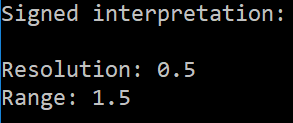
\includegraphics[scale=1]{../E1TP1/ejemploOutput}
\caption{\color{cyan}Output corresponding to the example input $"0\ 1\ 1"$.}
\label{image output}
\end{figure}

\subsection{\color{purple}Testing the Program}
%HACEEEEEEEEEEEEEEEEEEEEEEEEEEEEEEEEEEEEEEEEEEEER ESTA PARTEEEEEEEEEEEEEEEEEEEEEEEEEE

%\end{document}


%Información usada:

% beginners guide to latex:
% http://www.docs.is.ed.ac.uk/skills/documents/3722/3722-2014.pdf

% fixed point mathematics:
%http://fileadmin.cs.lth.se/cs/Education/EDA075/notes/mgh_appA_fixed.pdf

\section{\color{olive}Excercise 2: Simplification of a Maxterm Expression and its Corresponding Logical Circuit}

Having the function in maxterms $$f_1 (A,B,C,D) = \prod\left(M_0, M_1 , M_5 , M_7 , M_8 , M_{10} , M_{14} , M_{15} \right)$$ equivalent to $$f_2 (A,B,C,D) = \sum\left(m_2, m_3 , m_4 , m_6 , m_9 , m_{11} , m_{12} , m_{13} \right)$$ using minterms, can be simplified by different ways and represented using logic gates.

    \subsection{\color{purple}Simplification by Boolean Algebra}

    Using the Boolean algebra properties $$(A+B).(A+\overline{B})=A~(1)$$ or $$(AB)+(A\overline{B})=A~(2)$$ the function can be simplified using (1):
    \begin{eqnarray*}
        f_1 (A,B,C,D) &= &(A+B+C+D).(A+B+C+\overline{D}).(A+\overline{B}+C+\overline{D}).(A+\overline{B}+\overline{C}+\overline{D}).\\
        &&(\overline{A}+B+C+D).(\overline{A}+B+\overline{C}+D).(\overline{A}+\overline{B}+\overline{C}+D).(\overline{A}+\overline{B}+\overline{C}+\overline{D}) \\
        &=&(A+B+C).(A+\overline{B}+\overline{D}).(\overline{A}+B+D).(\overline{A}+\overline{B}+\overline{C})
    \end{eqnarray*}
    Which in minterms would be, using (2):
    \begin{eqnarray*}
        f_2(A,B,C,D) &= &(\overline{A}\overline{B}C\overline{D})+(\overline{A}\overline{B}CD)+(\overline{A}B\overline{C}\overline{D})+(\overline{A}BC\overline{D})+\\
        &&(A\overline{B}\overline{C}D)+(A\overline{B}CD)+(AB\overline{C}\overline{D})+(AB\overline{C}D)\\
        &=&(A\overline{B}D)+(\overline{A}B\overline{D})+(\overline{A}\overline{B}C)+(AB\overline{C})
    \end{eqnarray*}

    \subsection{\color{purple}Simplification by Karnaugh Map}

    A Karnaugh map is an easier way to simplify logic expressions when the function is too complex or too large to handle, because the Karnaugh map gives a more representative view for a faster analysis.

    If the simplification is done with minterms, the groups should be of ones and powers of 2, adding each group in case there is more than one, and in each group the independent variables would be multiplied.
    \begin{center}
        \begin{Karnaugh}
            %cada 4 es una fila, la col 3 es la 4ta columna y 3fila es la 4 fila
            \contingut{
            0,1,0,1,
            0,0,1,1,
            1,1,0,0,
            1,0,1,0}
            \implicant{6}{14}{red}
            \implicant{3}{7}{green}
            \implicant{12}{8}{orange}
            \implicantdaltbaix[3pt]{1}{9}{blue}
            %\implicantcantons[2pt]{orange}
            %\implicantcostats{4}{14}{green}
        \end{Karnaugh}
    \end{center}

    Now grouping by colours we get that the function in minterms would be:
    \begin{eqnarray*}
        f_2(A,B,C,D)&=&(A\overline{B}D)~(Red)\\
        &&+(\overline{A}B\overline{D})~(Blue)\\
        &&+(\overline{A}\overline{B}C)~(Orange)\\
        &&+(AB\overline{C})~(Green)
    \end{eqnarray*}

    The same method could be done with maxterms; grouping zeroes in powers of 2, then multipling groups in case there is more than one, and in each group the independent variables would be added.

    \subsection{\color{purple}Logic Circuit: AND, OR and NOT}

    Using the logic gates AND, OR and NOT the simplified version of the function could be represented by the figure below:

    \begin{figure}[htb!]
        \centering
        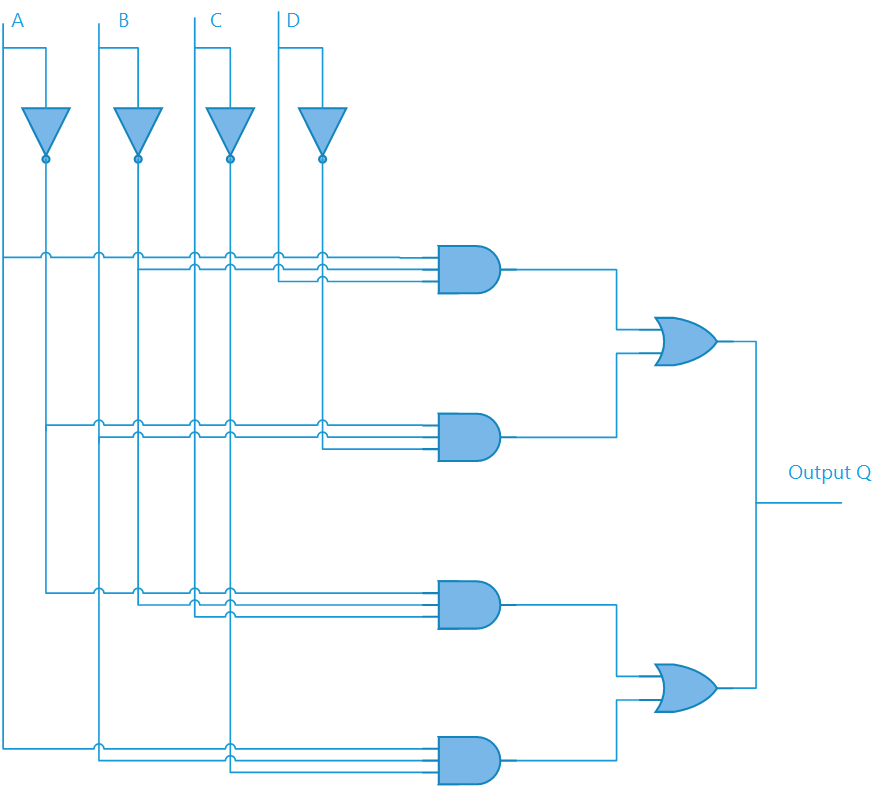
\includegraphics[scale=0.45]{../E2TP1/normallogic.png}
        \caption{\color{cyan}Logic circuit using AND, OR and NOT gates}
        \label{fig:normllogic}
    \end{figure}

    \pagebreak

    \subsection{\color{purple}Logic Circuit: NAND}

    All the gates used above could be equivalent to a combination of NAND or NOR gates. Therefore, the simplified function can be drawn as the next figure:

    \begin{figure}[h!]
        \centering
        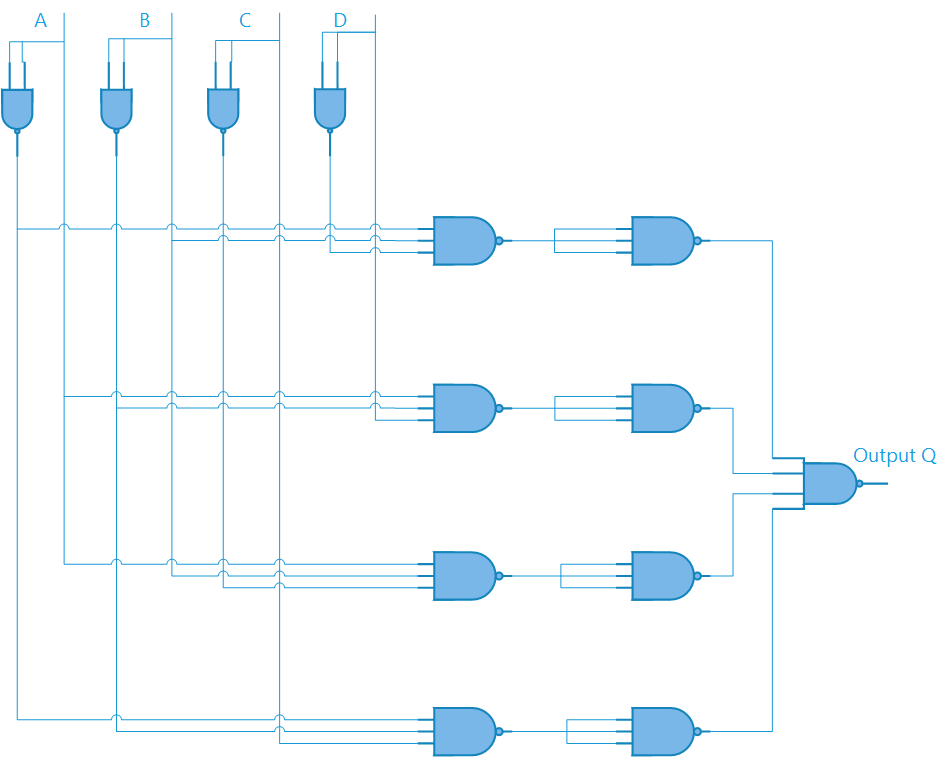
\includegraphics[scale=0.45]{../E2TP1/nandlogic.png}
        \caption{\color{cyan}Logic circuit using NAND gates}
        \label{fig:nandlogic}
    \end{figure}

\section{\color{olive}Excercise 3: Four-Entry Encoder and Four-Output Demux using Verilog}
Implement the following modules in Verilog:
\begin {itemize}
\item 4 inputs \textsc{encoder}
\item 4 outputs \textsc{demux}
\end {itemize}

\subsection{\color{purple}4-Input ENCODER}
\subsubsection{\color{orange}Description}
An encoder is an Application-Specific Integrated Circuit (ASIC) that converts information. In this case it receives a signal from  a 4-bit input and returns the position of the Most Significant Bit that is currently on.
\subsubsection{\color{orange}Code Implementation}
The Code Implementation of both the Module and its testbench can be found in their respective directories.
\subsubsection{\color{orange}Module Tests}
\label{subsec1}
Testbench results can be found in Table \ref{subsec1}
\begin{center}
\begin{tabular}{|c|c|c|}
\hline
Input&Output&Value\\
\hline
0001&00&0\\
0010&01&1\\
0100&10&2\\
1000&11&3\\
0011&01&1\\
0101&10&2\\
1001&11&3\\
0110&10&2\\
1010&11&3\\
1100&11&3\\
\hline
\end{tabular}
\\\vspace{12pt}
Table \ref{subsec1} \textsc{encoder} Testbench Results
\end{center}

\subsubsection{\color{orange}Conclusions}
The module is working as expected, where it is taking only the Most Significant Bit as the value to be encoded.

\subsection{\color{purple}4-output DEMUX}

\subsubsection{\color{orange}Description}
A DEMUX is an ASIC which receives an input signal and a selector signal. The selector signal determines through which output port the input signal is sent.

\subsubsection{\color{orange}Code Implementation}
The Code implementation for the \textsc{demux} can be found in its corresponding folder.

\subsubsection{\color{orange}Module Tests}
\label{subsec2}

\begin{center}
\begin{tabular}{|c|c|c|c|c|c|}
\hline
Input&Selector&Out\_0&Out\_1&Out\_2&Out\_3\\
\hline
1&0&1&0&0&0\\
1&1&0&1&0&0\\
1&2&0&0&1&0\\
1&3&0&0&0&1\\
\hline
\end{tabular}
\\\vspace{12pt}
Table \ref{subsec2} \textsc{demux} Testbench Results
\end{center}

\subsubsection{\color{orange}Conclusions}
The module works as expected.
%% LyX 2.2.3 created this file.  For more info, see http://www.lyx.org/.
%% Do not edit unless you really know what you are doing.
\documentclass[english]{article}
\usepackage[T1]{fontenc}
\usepackage[latin9]{inputenc}
\usepackage{geometry}
\geometry{verbose,tmargin=3cm,bmargin=3cm,lmargin=3cm,rmargin=3cm,headheight=3cm,headsep=3cm}
\usepackage{float}
\usepackage{graphicx}

\makeatletter

%%%%%%%%%%%%%%%%%%%%%%%%%%%%%% LyX specific LaTeX commands.
%% Because html converters don't know tabularnewline
\providecommand{\tabularnewline}{\\}

\makeatother

\usepackage{babel}
\begin{document}

\title{Electr�nica III TP1}
\maketitle

\section{Ejercicio 4}

\begin{figure}[H]
\begin{centering}
\begin{tabular}{|c|c|c|c|c|c|c|c|}
\hline 
$x_{1}$ & $x_{2}$ & $x_{3}$ & $x_{4}$ & $f_{1}$ & $f_{2}$ & $f_{3}$ & $f_{4}$\tabularnewline
\hline 
\hline 
0 & 0 & 0 & 0 & 0 & 0 & 0 & 1\tabularnewline
\hline 
0 & 0 & 0 & 1 & 1 & 1 & 1 & 1\tabularnewline
\hline 
0 & 0 & 1 & 0 & 1 & 1 & 1 & 0\tabularnewline
\hline 
0 & 0 & 1 & 1 & 1 & 1 & 0 & 1\tabularnewline
\hline 
0 & 1 & 0 & 0 & 1 & 1 & 0 & 0\tabularnewline
\hline 
0 & 1 & 0 & 1 & 1 & 0 & 1 & 1\tabularnewline
\hline 
0 & 1 & 1 & 0 & 1 & 0 & 1 & 0\tabularnewline
\hline 
0 & 1 & 1 & 1 & 1 & 0 & 0 & 1\tabularnewline
\hline 
1 & 0 & 0 & 0 & 1 & 0 & 0 & 0\tabularnewline
\hline 
1 & 0 & 0 & 1 & 0 & 1 & 1 & 1\tabularnewline
\hline 
1 & 0 & 1 & 0 & 0 & 1 & 1 & 0\tabularnewline
\hline 
1 & 0 & 1 & 1 & 0 & 1 & 0 & 1\tabularnewline
\hline 
1 & 1 & 0 & 0 & 0 & 1 & 0 & 0\tabularnewline
\hline 
1 & 1 & 0 & 1 & 0 & 0 & 1 & 1\tabularnewline
\hline 
1 & 1 & 1 & 0 & 0 & 0 & 1 & 0\tabularnewline
\hline 
1 & 1 & 1 & 1 & 0 & 0 & 0 & 1\tabularnewline
\hline 
\end{tabular}
\par\end{centering}
\caption{Complemento a 2 de los bits de entrada}
\end{figure}

Si escribimos cada bit de salida en funci�n de los mint�rminos de
los bits de entrada, nos quedan las siguientes ecuaci�nes:
\begin{center}
$f_{1}(m_{i})=m_{1}+m_{2}+m_{3}+m_{4}+m_{5}+m_{6}+m_{7}+m_{8}$
\par\end{center}

\begin{center}
$f_{2}(m_{i})=m_{1}+m_{2}+m_{3}+m_{4}+m_{9}+m_{10}+m_{11}+m_{12}$
\par\end{center}

\begin{center}
$f_{3}(m_{i})=m_{1}+m_{2}+m_{5}+m_{6}+m_{9}+m_{10}+m_{13}+m_{14}$
\par\end{center}

\begin{center}
$f_{4}(m_{i})=m_{0}+m_{1}+m_{3}+m_{5}+m_{7}+m_{9}+m_{11}+m_{13}+m_{15}$
\par\end{center}

Remplazando los valores de cada mintermino, quedan las siguientes
formulas:
\begin{center}
$f_{1}(x_{1};x_{2};x_{3};x_{4})=\bar{x_{1}}\bar{x_{2}}\bar{x_{3}}x_{4}+\bar{x_{1}}\bar{x_{2}}x_{3}\bar{x_{4}}+\bar{x_{1}}\bar{x_{2}}x_{3}x_{4}+\bar{x_{1}}x_{2}\bar{x_{3}}\bar{x_{4}}+\bar{x_{1}}x_{2}\bar{x_{3}}x_{4}+\bar{x_{1}}x_{2}x_{3}\bar{x_{4}}+\bar{x_{1}}x_{2}x_{3}x_{4}+x_{1}\bar{x_{2}}\bar{x_{3}}\bar{x_{4}}$
\par\end{center}

\begin{center}
$f_{2}(x_{1};x_{2};x_{3};x_{4})=\bar{x_{1}}\bar{x_{2}}\bar{x_{3}}x_{4}+\bar{x_{1}}\bar{x_{2}}x_{3}\bar{x_{4}}+\bar{x_{1}}\bar{x_{2}}x_{3}x_{4}+\bar{x_{1}}x_{2}\bar{x_{3}}\bar{x_{4}}+x_{1}\bar{x_{2}}\bar{x_{3}}x_{4}+x_{1}\bar{x_{2}}x_{3}\bar{x_{4}}+x_{1}\bar{x_{2}}x_{3}x_{4}+x_{1}x_{2}\bar{x_{3}}\bar{x_{4}}$
\par\end{center}

\begin{center}
$f_{3}(x_{1};x_{2};x_{3};x_{4})=\bar{x_{1}}\bar{x_{2}}\bar{x_{3}}x_{4}+\bar{x_{1}}\bar{x_{2}}x_{3}\bar{x_{4}}+\bar{x_{1}}x_{2}\bar{x_{3}}x_{4}+\bar{x_{1}}x_{2}x_{3}\bar{x_{4}}+x_{1}\bar{x_{2}}\bar{x_{3}}x_{4}+x_{1}\bar{x_{2}}x_{3}\bar{x_{4}}+x_{1}x_{2}\bar{x_{3}}x_{4}+x_{1}x_{2}x_{3}\bar{x_{4}}$
\par\end{center}

\begin{center}
$f_{4}(x_{1};x_{2};x_{3};x_{4})=\bar{x_{1}}\bar{x_{2}}\bar{x_{3}}\bar{x_{4}}+\bar{x_{1}}\bar{x_{2}}\bar{x_{3}}x_{4}+\bar{x_{1}}\bar{x_{2}}x_{3}x_{4}+\bar{x_{1}}x_{2}\bar{x_{3}}x_{4}+\bar{x_{1}}x_{2}x_{3}x_{4}+x_{1}\bar{x_{2}}\bar{x_{3}}x_{4}+x_{1}\bar{x_{2}}x_{3}x_{4}+x_{1}x_{2}\bar{x_{3}}x_{4}+x_{1}x_{2}x_{3}x_{4}$
\par\end{center}

Si simplificamos cada ecuaci�n, se puede llegar a las siguientes expresiones:
\begin{center}
$f_{1}(x_{1};x_{2};x_{3};x_{4})=x_{1}\bar{x_{2}}\bar{x_{3}}\bar{x_{4}}+\bar{x_{1}}(x_{2}+x_{3}+x_{4})$
\par\end{center}

\begin{center}
$f_{2}(x_{1};x_{2};x_{3};x_{4})=x_{2}\bar{x_{3}}\bar{x_{4}}+\bar{x_{2}}(x_{3}+x_{4})$
\par\end{center}

\begin{center}
$f_{3}(x_{1};x_{2};x_{3};x_{4})=x_{3}\bar{x_{4}}+\bar{x_{3}}x_{4}$
\par\end{center}

\begin{center}
$f_{4}(x_{1};x_{2};x_{3};x_{4})=x_{4}+\bar{x_{1}}\bar{x_{2}}\bar{x_{3}}$
\par\end{center}

Al intentar expresar dichas formulas en graficos de compuertas logicas,
se consiguieron los siguientes:

\begin{figure}[H]
\begin{centering}
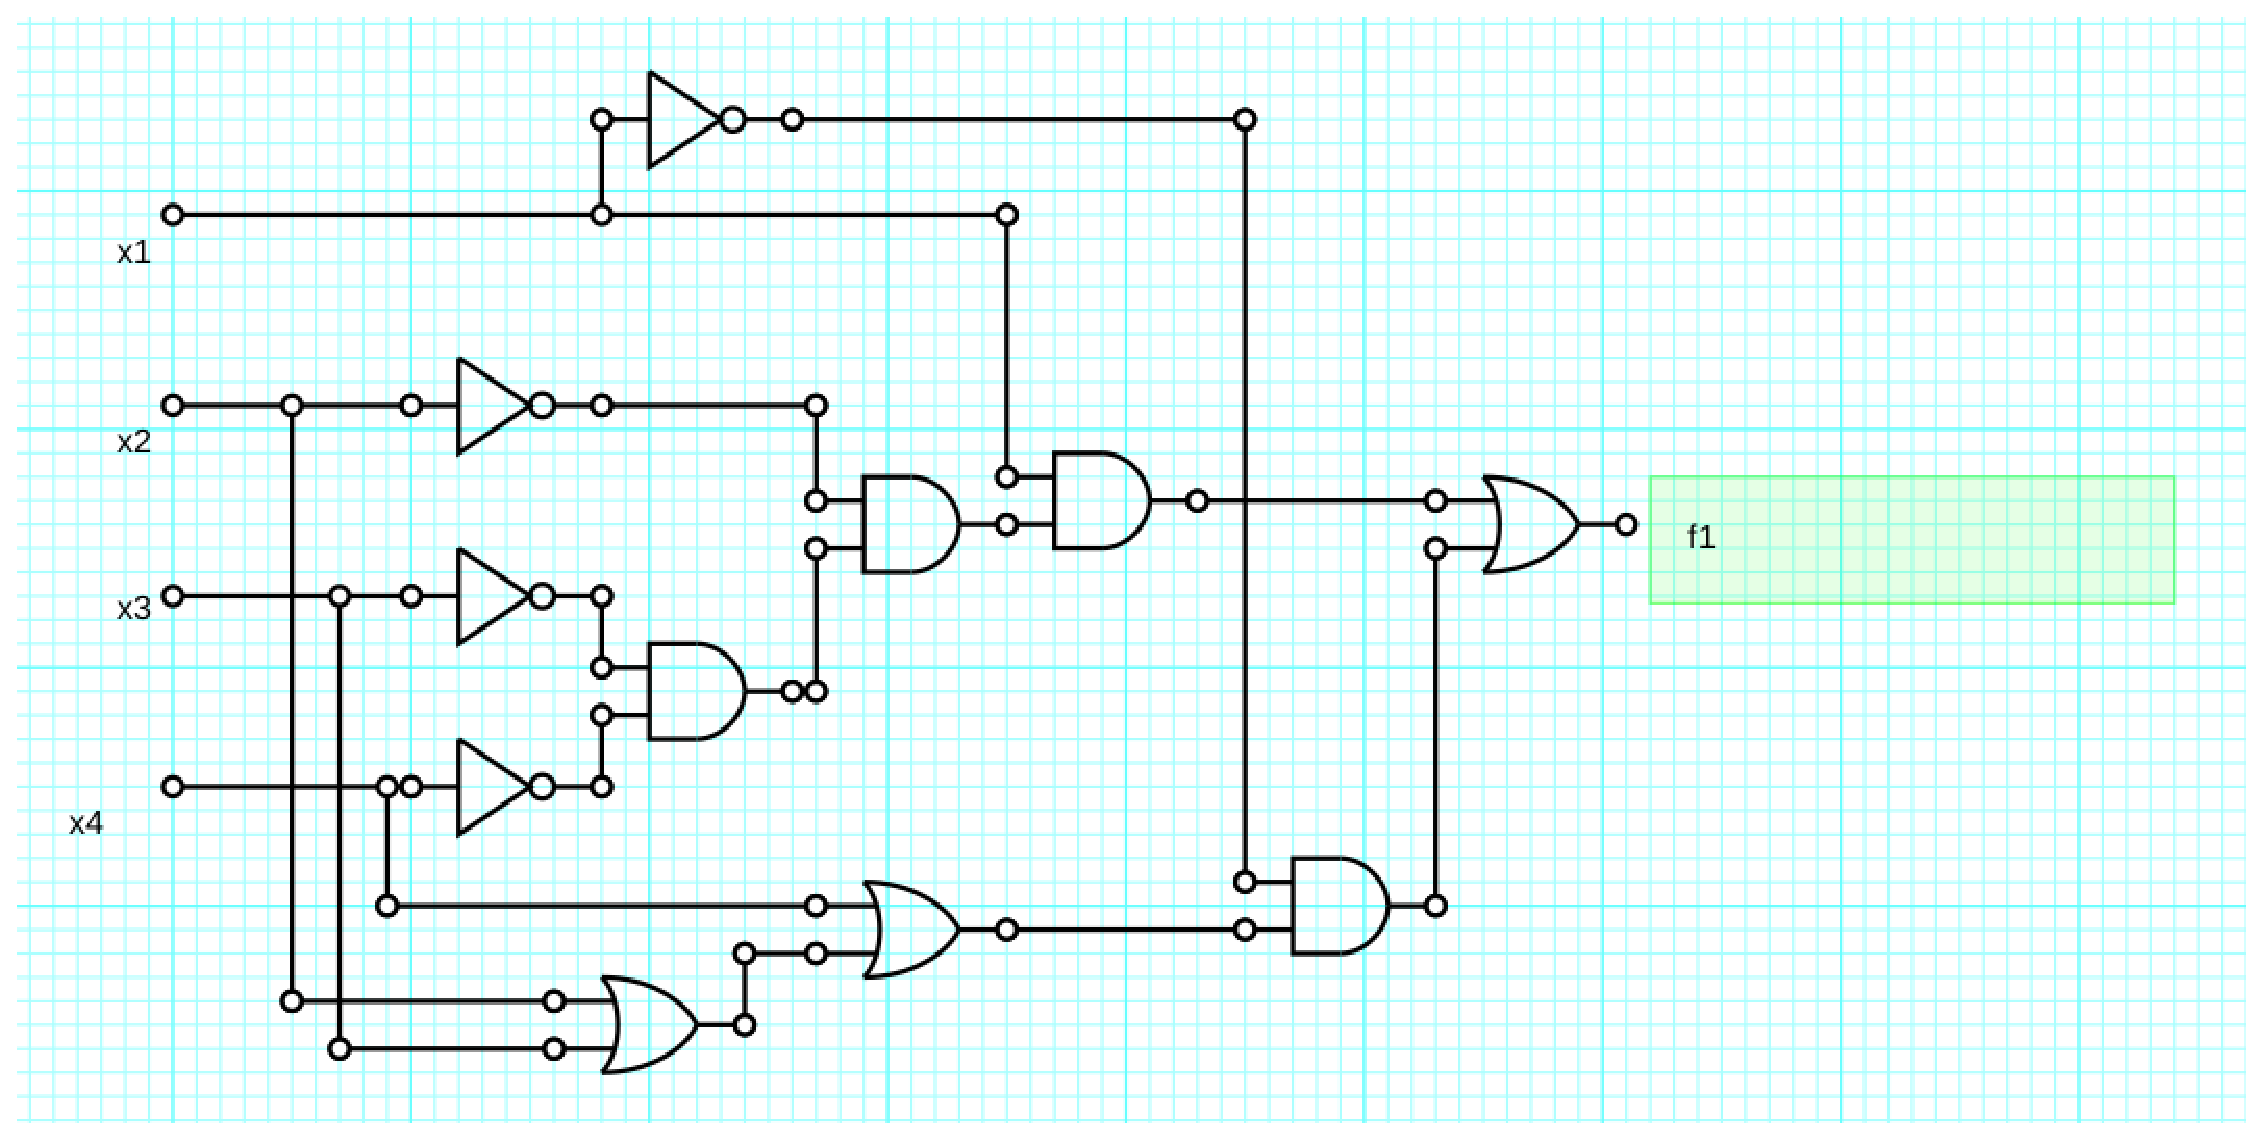
\includegraphics[scale=0.35]{images/1}
\par\end{centering}
\caption{Grafico de compuertas logicas Bit 1}

\end{figure}

\begin{figure}[H]
\begin{centering}
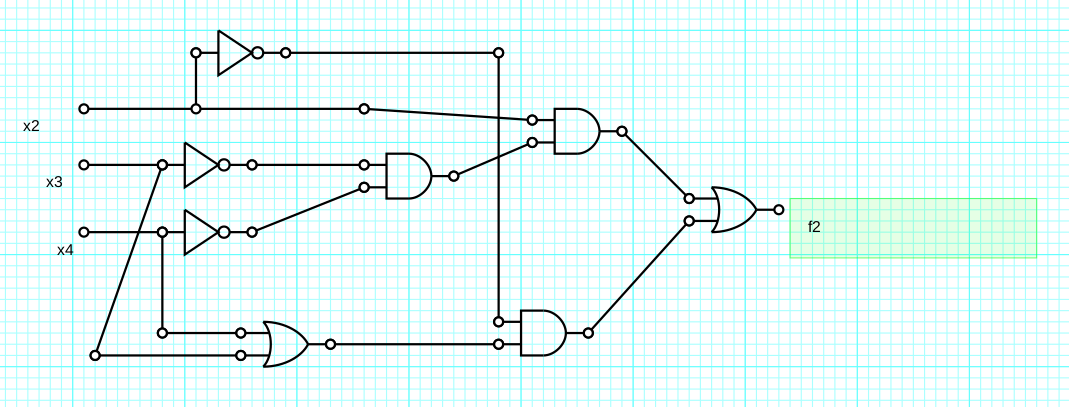
\includegraphics[scale=0.35]{images/2}
\par\end{centering}
\caption{Grafico de compuertas logicas Bit 2}
\end{figure}

\begin{figure}[H]
\begin{centering}
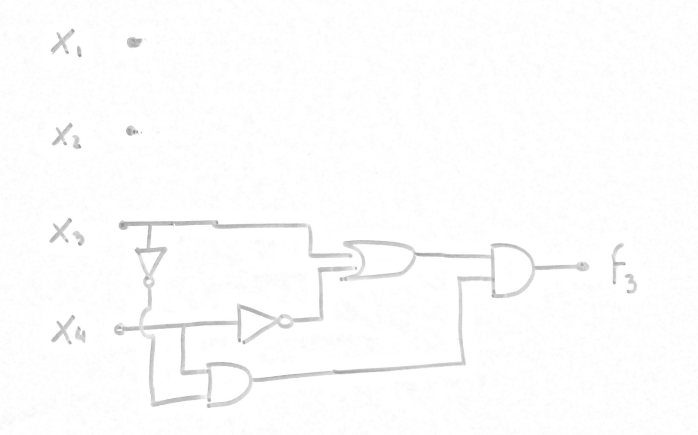
\includegraphics[scale=0.35]{images/3}
\par\end{centering}
\caption{Grafico de compuertas logicas Bit 3}
\end{figure}

\begin{figure}[H]
\begin{centering}
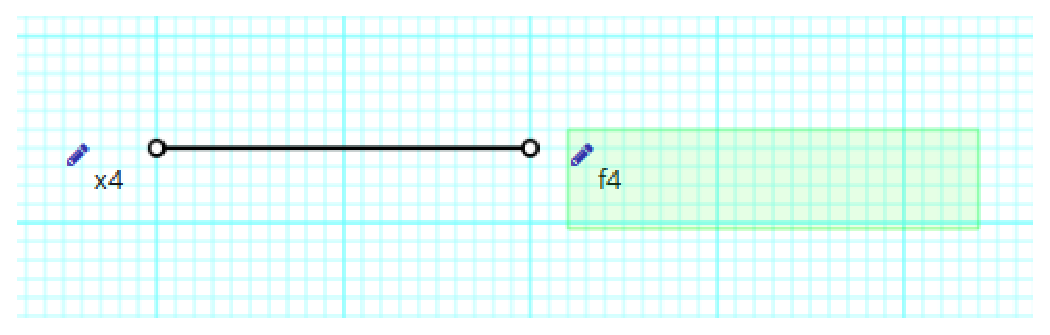
\includegraphics[scale=0.35]{images/4}
\par\end{centering}
\caption{Grafico de compuertas logicas Bit 4}
\end{figure}

Finalmente, esta logica de compuertas fue implementada en verilog
de la siguiente manera:

\begin{figure}[H]
\begin{centering}
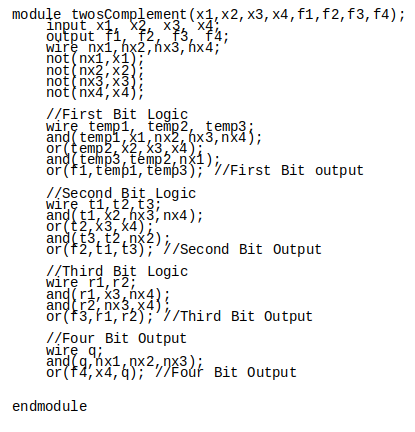
\includegraphics[scale=0.5]{images/5}
\par\end{centering}
\caption{Implementacion de la logica en Verilog}

\end{figure}

y al probar el codigo con un test.v se obtuvo la siguiente salida,
confirmando que el codigo se realizo de manera exitosa.

\begin{figure}[H]
\begin{centering}
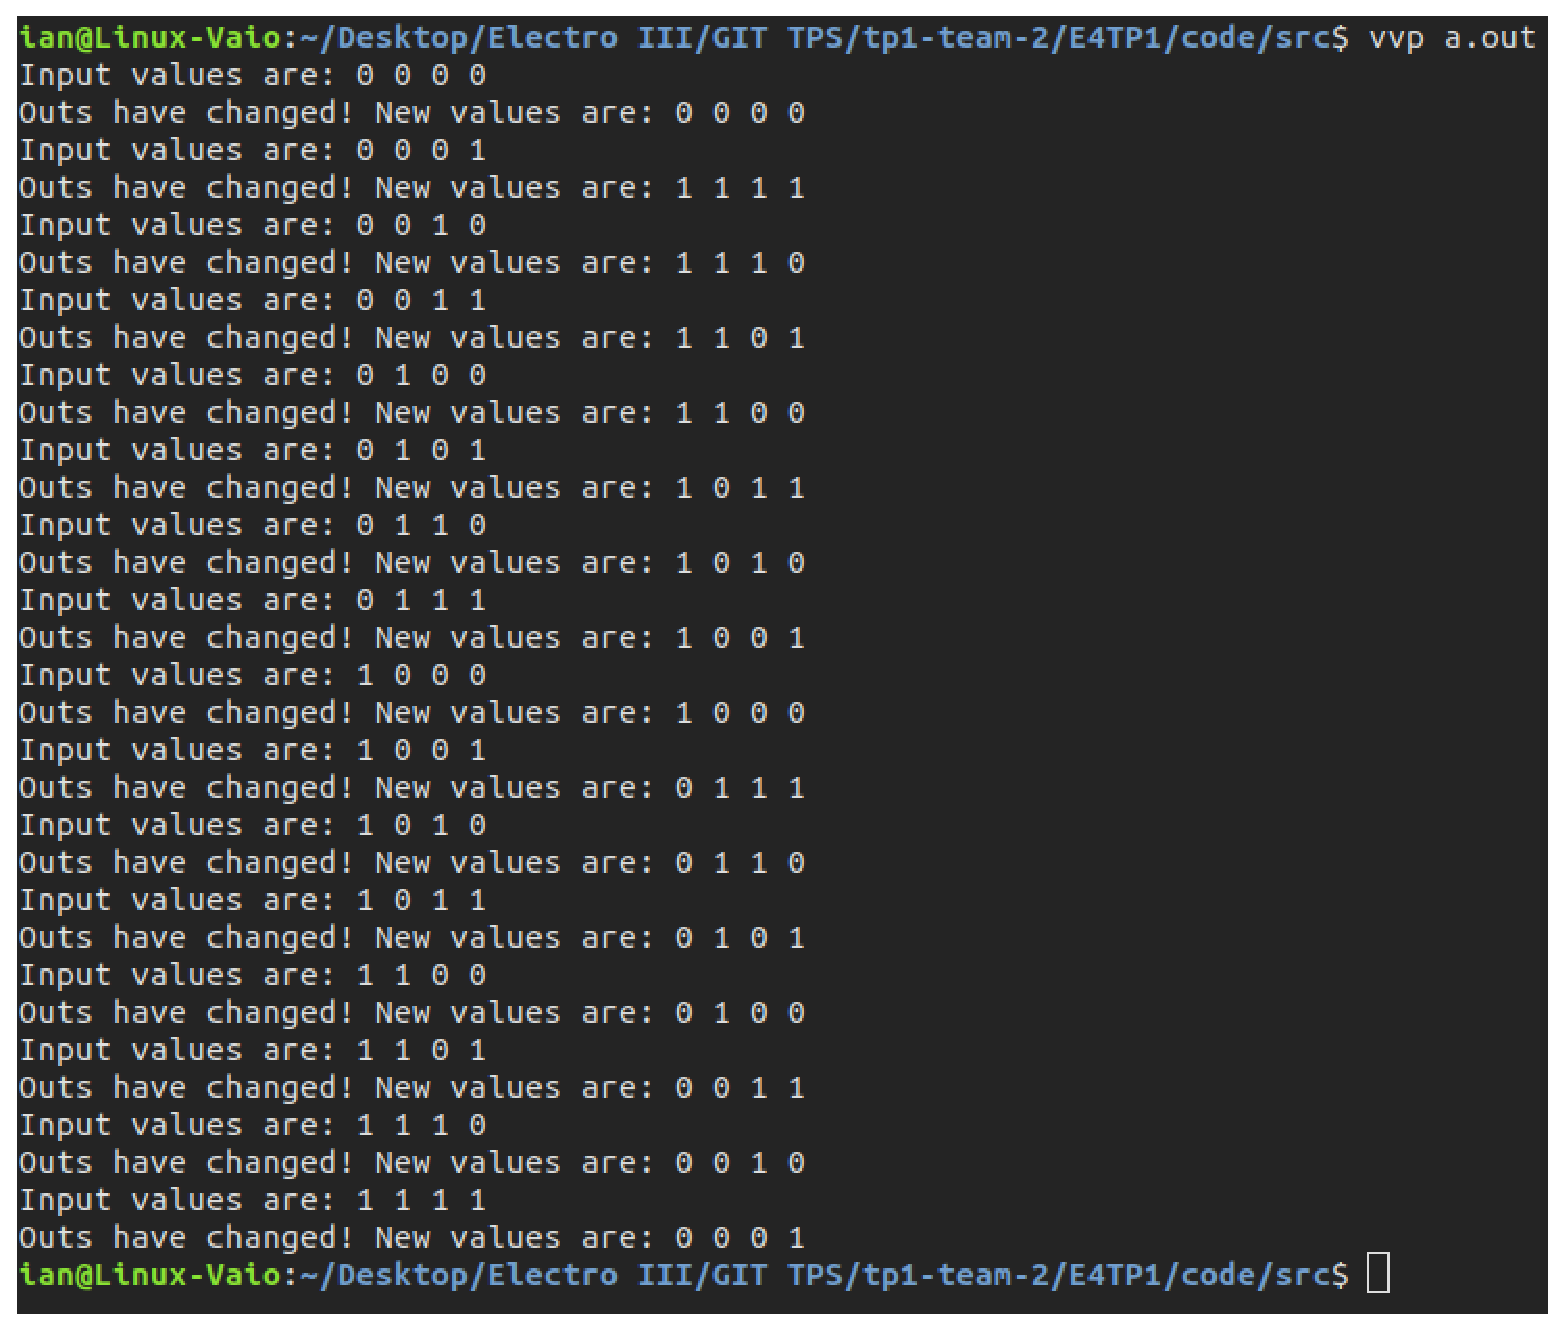
\includegraphics[scale=0.5]{images/6}
\par\end{centering}
\caption{Salida de la implementacion en la Terminal}

\end{figure}


\end{document}

%\section {\color{olive}Excercise 5: BCD Format Adder}
A module that receives as inputs two one-digit numbers in Binary-Coded-Decimals (BCD) format and outputs a two-digit number in BCD format, is implemented.

\subsection{\color{purple}Design Considerations}
\begin{itemize}
\item BCD digits are formed by 4 bits with a range of integer values between 0 and 9. Any value outside that range should be considered an error.
\item It needs to make a simple addition. Given that the maximum value of the sum is 18, the result will be a 5-bit integer.
\item The value of the sum must be returned in BCD format, so the 5-bit integer needs to be separated into 2 BCD digits.
\end{itemize}

Given these conditions, the module needs:
\begin{itemize}
\item 2 4-bit input ports
\item 2 4-bit output ports
\item 1 \textsc{error} register
\end{itemize}

\subsection{\color{purple}Code Implementation}
The BCD Adder was formed by the following modules:
\begin{itemize}
\item 2 BCD format "filters"
\item 1 4-bit numbers' adder
\item 1 BCD format "decoder"
\end{itemize}

The code implementation for each of the modules can be found in their respective folders in E5TP1/src.

\subsection{\color{purple}Module Testbench}
Testbench results for each submodule can be found in the directory /E5TP1/tests.txt.\\
Testbench results for the main module can be found in the directory /E5TP1/final.txt.

\subsection{\color{purple}Conclusions}
Each sub-module is working as intended, and so the final module works as intended: returning the sum of
the BCD format numbers and indicating whether the received input is valid or not.



\section{\color{olive}Excercise 6: ALU Implementation}

For this exercise we were asked to implement a 4 bit Aritmetic Logic
Unit (ALU). The operations we had to develop were SUM, SUBSTRACTION,
AND, OR, NOT, XOR, two's complement and shift left. In order to do this, we decided
to create a module responsible of adding 2 bits, and as output, it
returned 2 bits, one bit for the answer, and another for the carry
bit. By using this module, we then decided to create a secondary module,
responsible for adding 3 bits. This decision gave us al lot of simplification
in the development of the module SUM for 4 bits. As you can see in
the code "sum.v'' found in the folder src, we commented the previous
development without the module sum3Bits, and the new development with
the module sum3Bits.

For the substaction, we decided to re-use the module created on exercise
4 of two's complement, and utilizing it correctly with the module
SUM, we had our SUBSTRACTION module. For the operations AND, OR, NOT,
XOR we chosen to use the predefined modules provided by verilog and
utilize them bitwise.

\subsection{\color{purple}Definitions}

In this Aritmetic Logic Unit, we implemented with two accumulators
(that we will call A and B), each one of four bits, three operational
bits, four bits for the output accumulator (that we will call accumulator
C) and one carry bit, ordered in the way they were mentioned.

To select the operation you want to make, you should turn the three
operational bits in the following way:

\begin{table}[h!]
\begin{centering}
\begin{tabular}{|c|c|c|c|}
\hline 
 & Bit 0  & Bit 1  & Bit 2\tabularnewline
\hline 
\hline 
AND  & 0  & 0  & 0\tabularnewline
\hline 
NOT  & 0  & 0  & 1\tabularnewline
\hline 
OR  & 0  & 1  & 0\tabularnewline
\hline 
XOR  & 0  & 1  & 1\tabularnewline
\hline 
SHIFT LEFT  & 1  & 0  & 0\tabularnewline
\hline 
SUM  & 1  & 0  & 1\tabularnewline
\hline 
SUBSTRACTION  & 1  & 1  & 0\tabularnewline
\hline 
TWO'S COMPLEMENT  & 1  & 1  & 1\tabularnewline
\hline 
\end{tabular}
\par\end{centering}
\caption{Representation of operational bits}
\end{table}
\begin{itemize}
\item AND: Performs an AND operation bitwise between acummulators A and
B and returns it on accumulator C, meanwhile, the carry bit is left
to zero.
\item NOT: Performs a logic NOT operation bitwise between acummulators A
and B, and returns the answer in the accumulator C. The carry bit
stays as zero
\item OR: Performs a logic OR operation bitwise between accumulators A and
B, and returns the answer in the accumulator C. The carry bit stays
as zero.
\item XOR: Performs a logic XOR operation bitwise between accumulators A
and B, and returns the answer in the accumulator C. The carry bit
stays as zero.
\item SHIFT LEFT: It manages to move every bit in accumulator A, one space
left, and insterts a logic zero to the less significant bit. The answer
is given in the C acccumulator and the carry bit will become 0 or
1 dependig on the most significant bit of A.
\item SUM: Performs a numeric sum of the binary values of accumulator A
and B and the answer is given in accumulator C. Depending on the overflow,
the carry bit will become 1 or 0.
\item SUBSTRACTION: Performs a numeric substraction of the binary values
of accumulator A and B and the answer is given in accumulator C. The
carry bit will become 1.
\item TWO'S COMPLEMENT: Performs a two's complement of the binary value
of accumulator A and the answer is given in accumulator C. The carry
bit will become 0.
\end{itemize}




%%% End document
\end{document}
